\subsection{Composition viewpoint}

    \subsubsection{UML component diagram}
        \begin{figure}[!ht]
            \centering
            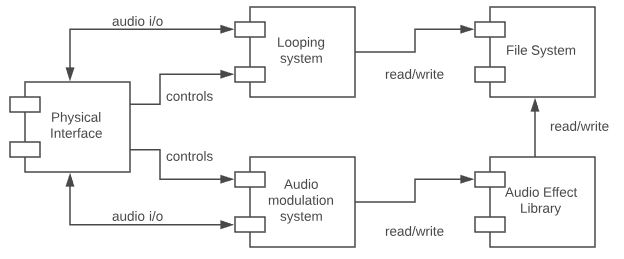
\includegraphics{diagrams/component-diagram.JPG}
            \caption{Component diagram}
            \label{fig:component}
        \end{figure}
    \subsubsection{Function attribute}
        The composition of the above entities creates the entire system to allow musicians to modulate incoming audio, or record and playback audio.
        
    \subsubsection{Subordinates attribute}
        The collection of the following entities work together to construct the working modulation/looping pedal: physical interface, looping system, audio modulation system, file system, and audio effect library.